\subsection*{\textbf{RQ6: To what extent do developers agree with our
		quantitative findings about delivery delay?}}

In this research question, we investigate how our participants feel about the
data that we collect during our prior quantitative studies
(\hyperref[st:study1]{Studies}~\ref{st:study1}, \ref{st:study2},
and~\ref{st:study3}). This research question
is divided into two subsections---one for each {\em theme} that is investigated
in this thesis---{\em (i)} delivery delay in general
and {\em (ii)} the impact of rapid release cycles on delivery delay
(\hyperref[fig:thesis_overview]{Figure}~\ref{fig:thesis_overview}).\\


\noindent\textit{\textbf{Theme~9---delivery delay in general.}}\theme{th:9}
In this analysis, we present the data that we collect in our prior studies
(\hyperref[ch:study12]{Chapter}~\ref{ch:study12}) and investigate if this data
resonates with participants' experience. We provide the methodology of our
data-related questions to participants through a web page that is mentioned in
our surveys (see~\hyperref[methodology:i]{Appendix}~\ref{methodology:i}).

\begin{figure}
	\centering
	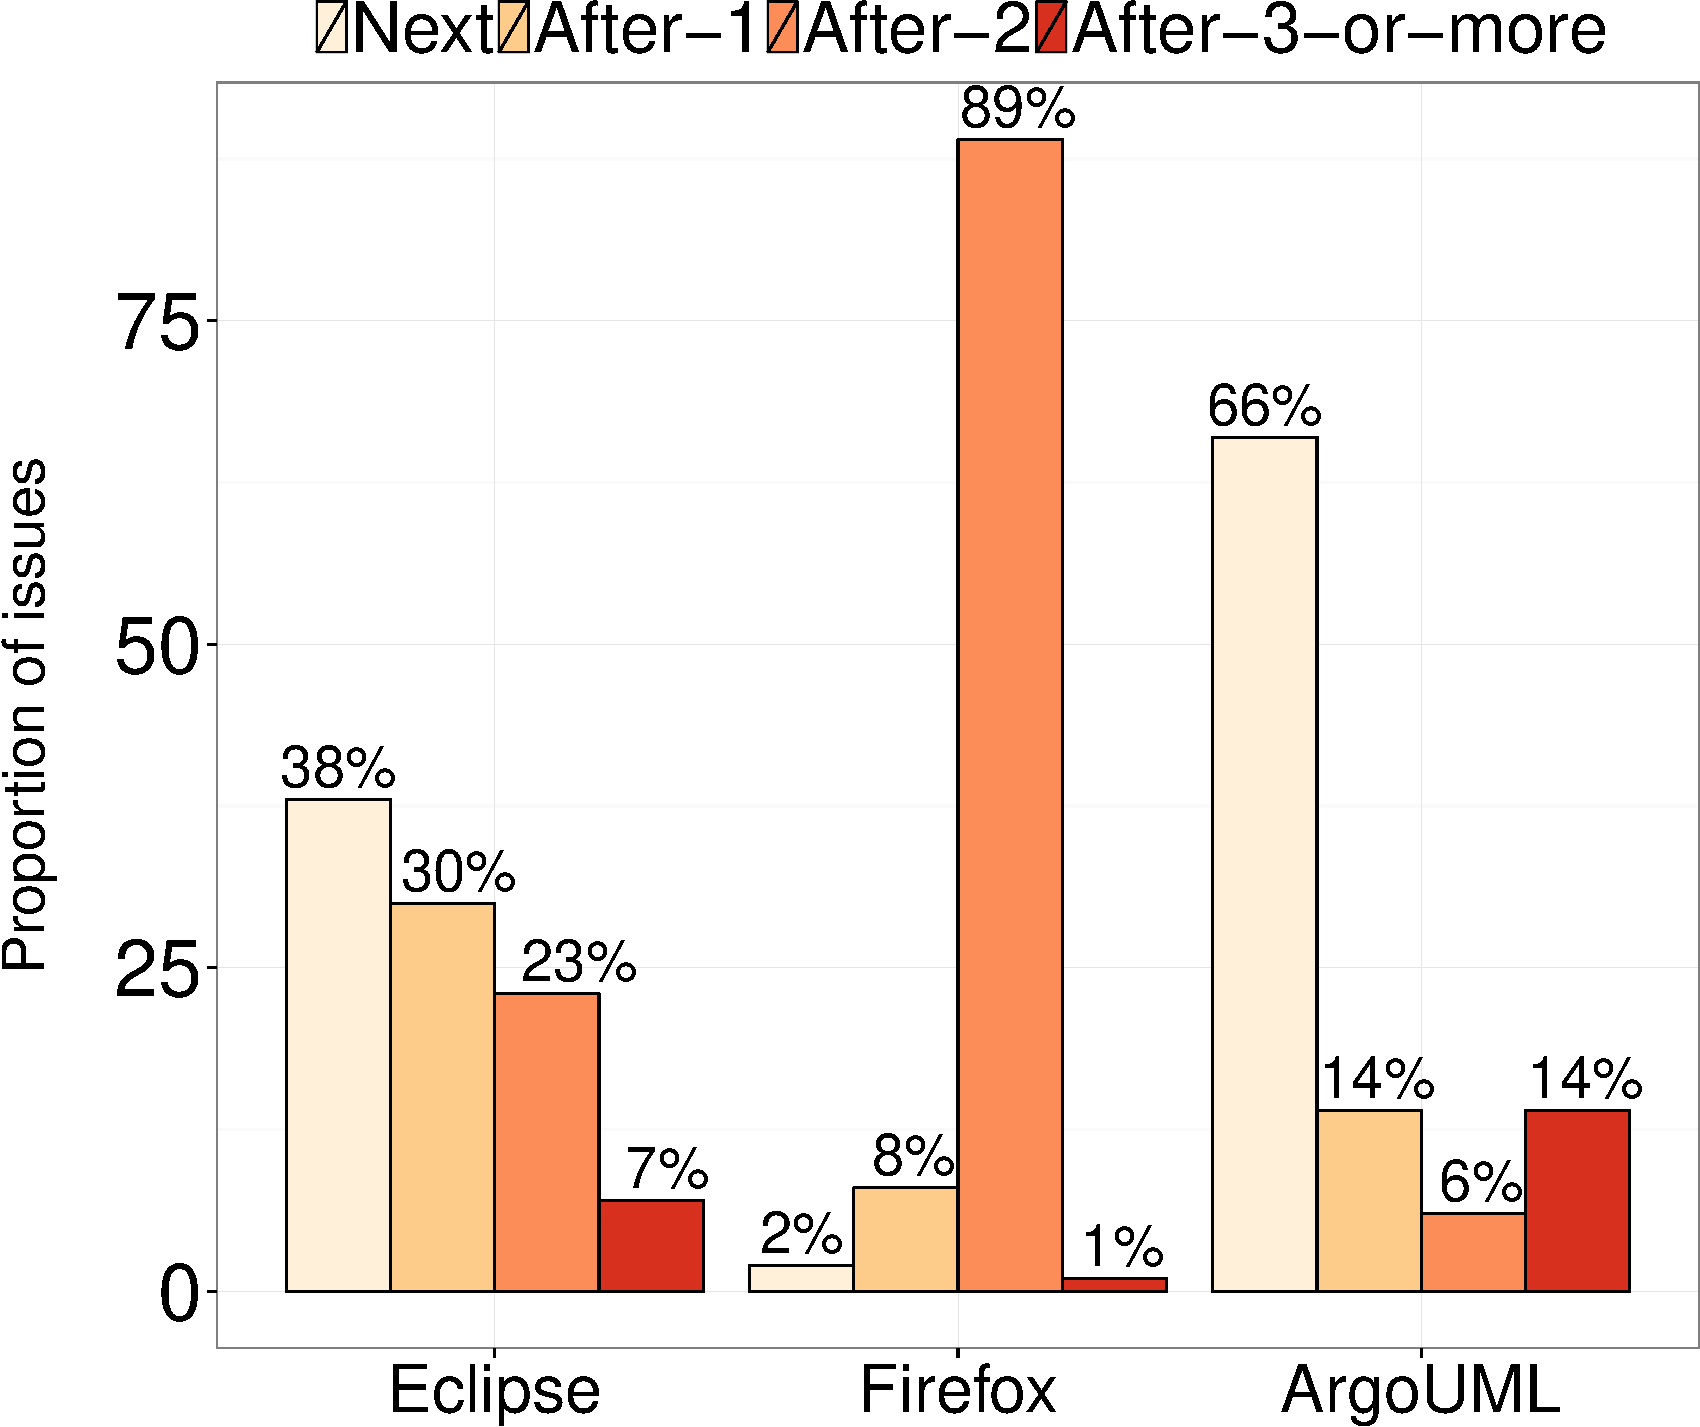
\includegraphics[width=0.80\textwidth,keepaspectratio]
	{chapters/chapter5/figures/rq6/datasets.pdf}
	\caption{Proportion of addressed issues that have their integration
		delayed by a given number of releases. For example, 89\% of the
	addressed issues skip two Firefox stable releases before being shipped
to users (this chart was already presented in
\hyperref[ch:study12]{Chapter}~\ref{ch:study12}. }
	\label{fig:data-related-rq1}
\end{figure}

\hyperref[fig:data-related-rq1]{Figure}~\ref{fig:data-related-rq1} shows the
chart that we presented to participants. For example, 89\% of the addressed
issues skip two Firefox stable releases before being shipped to users. The most
recurrent themes among the responses of participants to explain this data are:
{\em team workload}$^{(5)}$ and {\em dependency}.$^{(2)}$ Among the responses that
are related to {\em team workload},$^{(5)}$ {\em E27} explains that {\em
``committers  are too busy,''} while {\em E26} argues that there might be {\em
``delay[s] in review[s] when the issues [are] completed,''} which can generate
delivery delay. Regarding {\em dependency},$^{(2)}$ {\em E32}'s opinion is
that delivery delay may happen due to {\em ``the strong connection to other
Eclipse projects which makes integration more costly (time consuming).''}
Furthermore, two of our interviewees ({\em F11} and {\em F23}) provide us with
examples of why addressed issues may be delayed due to dependency problems. For
example, {\em F23} explains during the interview that delivery delay can
happen when there are {\em ``dependencies between projects and one of them gets
done, but the other implementation takes a longer while.''} Another example,
provided by {\em F23} is when {\em ``you release a bug fix but then you realize:
	Hey! These users are not able to use these websites anymore because web
	servers implement the spec in a wrong way or do some really weird things
that are not expected.''}

Additionally, we ask participants from the Eclipse and ArgoUML projects about
their opinion of why the data from the Firefox project behaves differently from
theirs, \ie a larger number of releases being skipped by addressed issues. The
most recurrent responses explain that this difference may be due to the {\em
	rapid release cycle}$^{(4)}$ that is adopted by the Firefox project. For
	example, {\em E30}'s opinion is that {\em ``on a rapid release cycle
		(e.g. 6 weeks for firefox), a two-release delay means 12 weeks,
		less than 3 months, which is still less than no delay for a fix
		submitted early in a project with a 6-month release cycle.''} 
\\           

\noindent\textit{\textbf{Theme~10---Impact of switching to a rapid release
cycle.}}\theme{th:10}
We present the data that is shown in
\hyperref[fig:traditional_vs_rapid]{Figure}~\ref{fig:traditional_vs_rapid} to
the participants of the Firefox project.
\hyperref[fig:traditional_vs_rapid]{Figure}~\ref{fig:traditional_vs_rapid}
compares the delivery delay between traditional and rapid release cycles. We
then ask if this result resonates with the participants' experience. More
details about how we show this data to participants can be found in
\hyperref[methodology:ii]{Appendix}~\ref{methodology:ii}. From the 14 responses that we received for this
question, 5 participants explicitly disagree with our analysis, while 6
participants explicitly agree with it. 

We interviewed two participants that disagree with the results ({\em F06} and
{\em F09}). After providing extra explanation about our methodology and asking
them to elaborate on their responses, we could better understand their reasons.
{\em F06} clarifies: {\em ``I'm not surprised that there are things in that
bucket''} (the short delays due to minor traditional releases), instead 
{\em ``I'm surprised that there are many of them.''} In addition, {\em F09} declared
{\em ``I misunderstood [your] question, but now it [(the data)] makes
sense.''} With respect to the remaining participants that disagree with our
results, they inform us that the data does not resonate with their experience. For
instance, {\em F21} provides the following opinion {\em ``this does not resonate
with my experience. I find the traditional model is much much slower than rapid
release to get fixes in users hands.''} 

From the set of participants that agree with our results, two of them explain
that the behaviour that is presented by the traditional release data is due to
the {\em integration rush}$^{(2)}$ that happens prior to shipping. {\em F15}'s
opinion is that {\em ``since missing a release cycle isn't a big deal, more
features are kept from being released until they're properly polished instead of
being rushed at the end of a long release cycle.''} {\em F22} also provides us
with a reasonable explanation when stating that our result {\em ``makes perfect
	sense as issues will, unless fast-tracked or held back, be released a
	set quantum of time after they are completed. This is dominated by the
	timing of the release schedule, not by the timing of the discovery or
fix.''}\\

\conclusionbox{The dependency of addressed issues on other projects and team
	workload are major perceived reasons to explain our findings about
	delivery delays. Moreover, participants are divided when explaining
	why traditional releases may have shorter delivery delays.
	Nevertheless, the fact that in rapid releases an integration rush is no
	longer needed and that additional time can be spent on polishing
	addressed issues emerge as main explanations as to why traditional
	releases can have shorter delivery delays.}

